\newpage
\section{PCB-Design und Layout}
Dieser Abschnitt beschreibt die praktische Umsetzung des Schaltplans auf der Leiterplatte. Im Gegensatz zum vorherigen Kapitel geht es hier nicht mehr um die Auswahl einzelner Bauteile, sondern um deren Platzierung, Verschaltung und elektrische Trennung im Layout.

Nach dem Schaltplanentwurf wurde das Layout der Leiterplatte erstellt. Dabei war es wichtig, die stromstarken Bereiche von den empfindlichen Logik- und Sensorschaltungen zu trennen. Die Bauteile wurden so platziert, dass die Stromversorgung kurze Wege zu den Verbrauchern hat und zusammengehörige Funktionsgruppen nah beieinander liegen.

Ein Schwerpunkt lag auf einer klaren Trennung zwischen Leistungsteil und Logikbereich sowie auf einer praktikablen Anordnung der Steckverbinder. Auch die Leitungsführung rund um den STM32 wurde so ausgelegt, dass die wichtigsten Signale möglichst direkt und übersichtlich geführt werden.

Die wichtigsten Bereiche des Layouts sind in Abbildung~\ref{fig:pcb-layout-bereiche} markiert.

\begin{figure}[H]
	\centering
	\begin{tikzpicture}
		\node[anchor=south west, inner sep=0] (board) at (0,0)
		{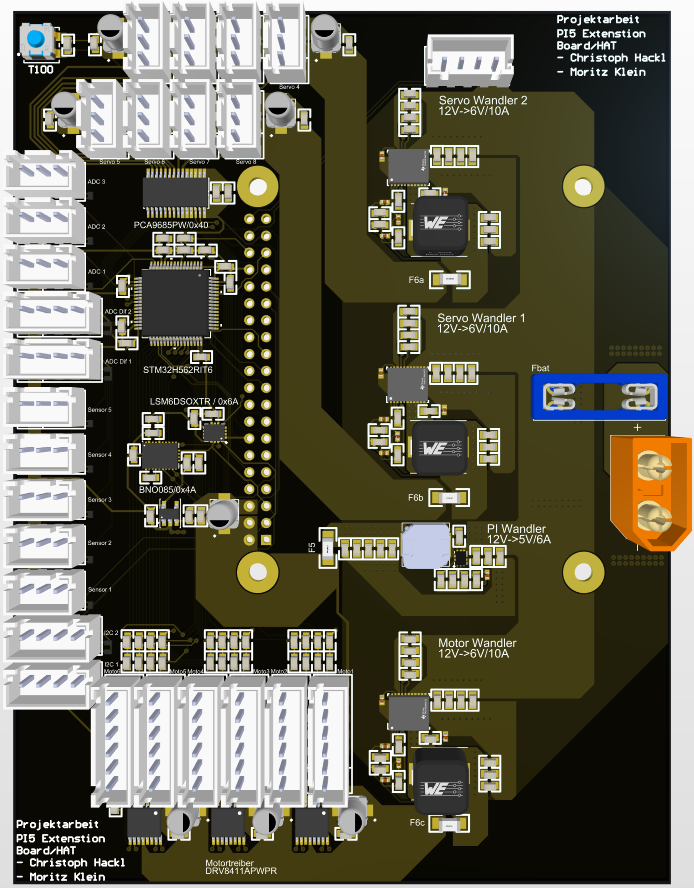
\includegraphics[width=0.7\linewidth]{Board.png}};
		\begin{scope}[x={(board.south east)}, y={(board.north west)}]
			\draw[red, very thick, fill=red!20, fill opacity=0.18]
			(0.53,0.05) rectangle (0.76,0.90);
			\node[draw=red, fill=white, rounded corners=2pt, font=\scriptsize, align=center]
			at (0.82,0.88) {Spannungs-\\wandler};

			\draw[blue, very thick, fill=blue!20, fill opacity=0.18]
			(0.15,0.38) rectangle (0.35,0.82);
			\node[draw=blue, fill=white, rounded corners=2pt, font=\scriptsize, align=center]
			at (0.25,0.66) {STM32 /\\Logik};

			\draw[green!50!black, very thick, fill=green!30, fill opacity=0.18]
			(0.09,0.82) rectangle (0.53,1);
			\node[draw=green!50!black, fill=white, rounded corners=2pt, font=\scriptsize, align=center]
			at (0.49,0.84) {Servo-\\bereich};

			\draw[orange, very thick, fill=orange!30, fill opacity=0.18]
			(0.15,0.00) rectangle (0.53,0.29);
			\node[draw=orange, fill=white, rounded corners=2pt, font=\scriptsize, align=center]
			at (0.33,0.31) {Motor-\\treiber};

			\draw[violet, very thick, fill=violet!25, fill opacity=0.18]
			(0.76,0.38) rectangle (1,0.58);
			\node[draw=violet, fill=white, rounded corners=2pt, font=\scriptsize, align=center]
			at (0.82,0.45) {Akku-\\eingang};

			\draw[cyan!60!black, very thick, fill=cyan!25, fill opacity=0.16]
			(0.00,0.20) rectangle (0.15,0.82);
			\node[draw=cyan!60!black, fill=white, rounded corners=2pt, font=\scriptsize, align=center]
			at (0.07,0.18) {Sensor-\\anschlüsse};

			\draw[magenta!80!black, very thick, fill=magenta!35, fill opacity=0.20]
			(0.35,0.38) rectangle (0.40,0.76);
			\node[draw=magenta!80!black, fill=white, rounded corners=2pt, font=\scriptsize, align=center]
			at (0.46,0.58) {Raspberry-\\Pi-Header};
		\end{scope}
	\end{tikzpicture}
	\caption{PCB-Layout mit markierten Spannungs- und Logikbereichen}
	\label{fig:pcb-layout-bereiche}
\end{figure}

